In this section we will start in the fundamental biological concepts before specializing in the [fruit fly]. We we will go through a short, broad explanation of the information YYY and how it is expressed. We will then talk about the fascinating biology that happens inside cells and during the creation of a [Drosophila]. Finally we will use all these newly learned concepts to introduce and biologically justify the model we have been working with. \\ \todo{rephrase}\\
Try to 3blue1brown' it:\\
By the end, we hope for every term and parameter to seem sensible and canonical in the way that we could have reinvented them for this thesis.


\section{Broken Symmetries and Genetic Patterning}
% \section{Everything}
\label{sec:theory-polarity}
\subsection{Broken Symmetries}

Almost all animals start as a single, isotropic sphere of cells. At one point, this ball will 'turn in on itself' and begin developing the organism to come. As animals are not spherically symmetric\footnote{except for your mom}, a number of symmetries need to be broken. 

In Drosophila Melongaster, after the first rounds of mitosis, the cells migrate to line the inside of their egg. This allows each of their surfaces to form distinct "outside" and "inside" domains. Through preferential adhesion\footnote{explain  preferential adhesion} based on their individual surface orientation, the cells can maintain the shell-form, thereby giving rise to the well-defined Inside-Outisde polarity. In biology this is known as Apical-Basal polarity and so universal it is seen in almost every multicellular system. 

Now, the fruit fly is cheating slightly, as its egg is oblong. This allows for the right/left-symmetry to be have been broken from birth.

Finally, we need some way of getting every cell to know the "forward" and "backward" directions. This polarity is called Planar-Cell-Polarity (for obvious reasons) and is almost as ubiquitous as the Apical-Basal polarity. The way the YYY zygote defines its YYY is through "the right hand rule" where a striped pattern .

The way these pattern emerge are fascinating! 



\subsection{Genetic Patterning}
\label{sec:gen_patterns}
For a multicellular organism to go from a single cell to forming the complex body plans we all know and love, some organizing is needed. This complicated interplay between cells necessitates are neihter controlled solely trhought the DNA nor "from the top"\todo{rephrase}. For humans and fruit fly alike, this is done via genetic patterning.\cite{veraksa2000developmental}

As predicted by Turing, patterning is a result of "smartly"\footnote{I know, I know, Nature abhors a vacuous anthropomorphization} designed interactions where different chemicals assists or inhibits the production or expression of each other. 

% Now, to shake it up, \textit{Twist} \& \textit{Snail}, which might remind you of the beetles,\footnote{The species \textit{Tribozium} for example\cite{sommer1994expression}} are vital for the early development of a surviving fruit fly.

Using a large bank of statistics, including the (normalized) expression, (the data and resources at \url{https://shiny.mdc-berlin.de/DVEX/}), we could map a lot of different YYY onto onto our YYY. 

TODO: Maybe explain data-processing?

This allowed us to group the cells after biologically defined type. Where we initially defined areas of interest after hand-drawn cell-fate maps, we can now specify boundaries between cell types on the unperturbed morphology the maternal gradients. A selection of some of the most important morphogens can be seen in Table \ref{tab:morphogens} (in Section \ref{App:morphogens} in the Appendix) and in Figure \ref{fig:MorphogenMap} their concentrations can be seen as mapped onto our virtual blastoderm.


\noindent

\begin{figure}[H]
    \centering
    \makebox[\linewidth]{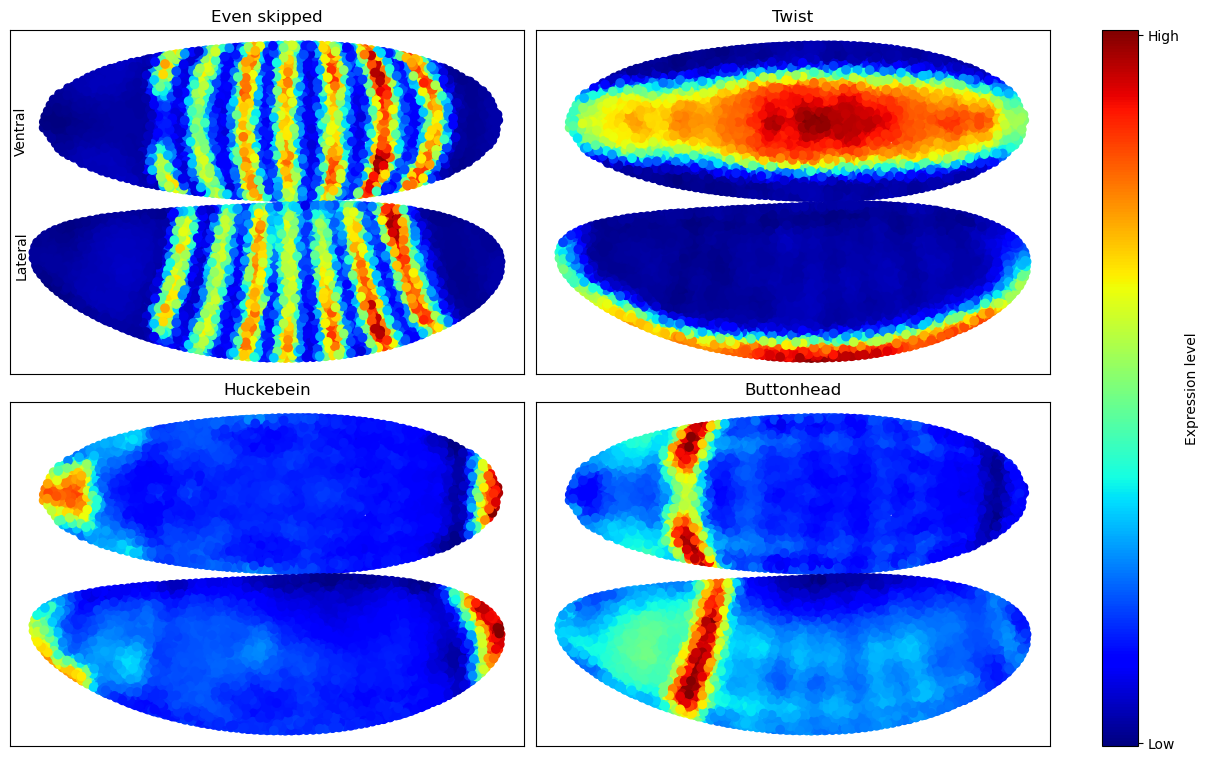
\includegraphics[width=1.2\linewidth]{chapters/Theory/figures/patterning.png}}
    \caption{The data extracted from \citeAY{shinyDVEX} as projected onto our embryo. A clear attest to the remarkable and stable pattern formation Turing predicted chemicals gradients capable of producing.}
    \label{fig:MorphogenMap}
\end{figure}


Now, these concentration gradients along with the aforementioned polarities allow for spatially complex, 

separately simple can apparently 

precise and robust macro scale morphology changes.


Importantly, the interaction between the morphogens and the mechanical deformations go both ways. It has been shown (J. Schauser et al) that a mechanical stimulus can trigger a chemical signal, thereby reinducing patterning in a feedback loop. This is called mechanotransduction and is believed to be vital in stable PCP-orientation. [citation needed] This means, that when the cells move according to some defined polarity, they can move the signal and break other cells' symmetries along the way. \todo{rephrase} Of course this requires them to be able to move, and how excactly they do that with neither legs nor wheels is explained here:\note{be serious } 


\section{How cells move}

Most of the global large-scale cell migration seen during development of multicellular organisms stem from a handful of seemingly simple\footnote{albeit still not well understood} active single-cell actions.\cite{walck2014cell}\\


The cells internal structure is called the cytoskeleton with internal \textit{motor proteins} responsible for keeping and changing the cells shape.

The motion we will be looking at, are of a type that is fundamentally different from Chemotaxis, with cells reacting to a local chemical concentration but not moving along a gradient [citation needed].

In general, in embryogenesis where cells are bound together in epithelial sheets, the cells are able to exert forces on each other. 
The global-scale changes in physical structure we will be exploring all arise from single cell actions with little to no discernible individual movement.

As can be seen on Figure \ref{fig:mysosinMeshwork}, the cells stay interconnected using membrane tethers connecting local neighborhoods. 

\begin{figure}[H]
    \centering
    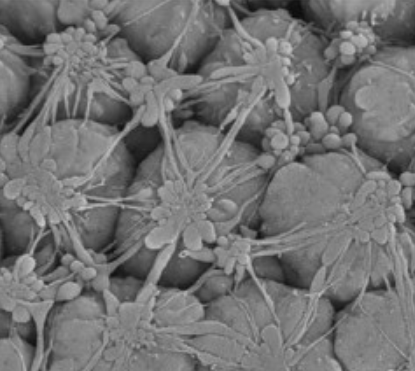
\includegraphics[width=0.6\linewidth]{chapters/Theory/figures/EM_constricting_proteins.png}
    \caption{Electron microscopy of Myosin II meshwork at ventral side. Taken from \citeAY{martin2010integration}}
    \label{fig:mysosinMeshwork}
\end{figure}

In Drosophila gastrulation, the role of these 'driving effects' are surprisingly under-understood with no paper claiming YYY with certainty.\footnote{This very much comes down to the fact, that experiments with living, moving cells are inherently intractable/hard} Here is a list of the fundamental single-cell active forces that is undeniably happening, even if not essential for the final outcome:\footnote{As nature is remarkably resilient, there is clear and definite evidence of one action overtaking when another fails to deliver. \textbf{Rewrite} This will be expanded upon in Section \ref{sec:mutantNoGB}} 

They are \textbf{Convergent Extension}, \textbf{Apical Constriction}, \textbf{Cell Shape Change} and \textbf{Proliferation}

\subsection{Convergent Extension}
\label{sec:ConvergentExtension}
For elongating of sheets in a single direction, \textit{Convergent Extension} seems to be one of the most common proprietors of movement. Consisting of asymmetric cellular intercolations, .



\begin{figure}[H]
    \centering
    \begin{subfigure}{0.45\linewidth}
        \centering
    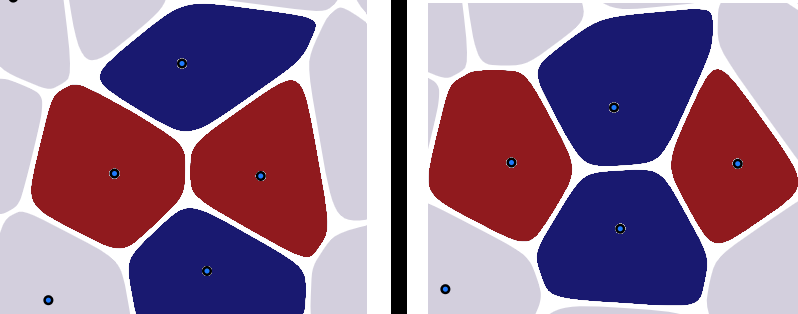
\includegraphics[width=\linewidth]{chapters/Theory/figures/ConvergentExtensionDiagram.png}
    \caption{A diagram showing how guided intercolation results in directional elongation}
    \end{subfigure}
        \begin{subfigure}{0.45\linewidth}
        \centering
        \caption{Dyed Germ Band tissue showing clear difference in horizontal and vertical protein expressions}
    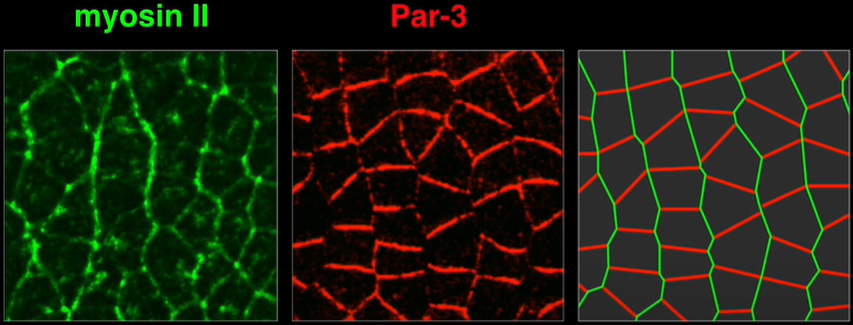
\includegraphics[width=\linewidth]{chapters/Theory/figures/bipolar-PCP.png}
    \end{subfigure}
    \caption{\cite{zallen2004patterned}\url{https://www.youtube.com/watch?v=MO7x7R-m3Qk}}
    
    \label{fig:ConvergentExtensionDiagram}
\end{figure}

The full [smth]-scale can change shape without the individual cells looking any different or needing to know their position in space. 

Wieshaus and [hende damen der] showed through laser ablation, Cell Intecolation. Anisotropic constriction of cell borders with deformations only happening  



We know that the signaling protein Wnt plays an important role in controlling Convergent Extension. For interesting writing, here is some foreshadowing: Wnt is also known as an inducer of Planar-Cell-Polarity.

\subsection{ Apical Constriction }
\label{sec:ApicalConstriction}
When the cell sheet wants out-of-plane bending, they turn to Apical Constriction. Apical constriction functions exactly as you would think; Myosin rings constrict the apical (outer) side of the cell, creating a smaller surface area. This leads to bending and, when enough constriction is applied, invagination. (see Figure \ref{fig:apical-constriction}). Cells has been shown the ability to constrict both isotropically and anisotropically.

\begin{figure}[H]
    \centering
    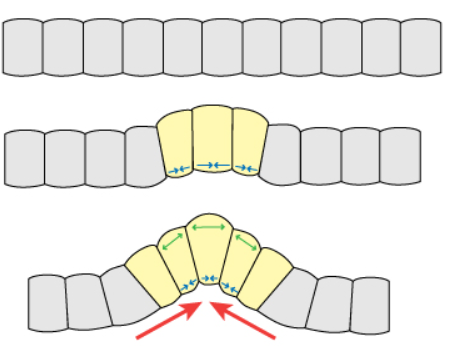
\includegraphics[width=0.3\linewidth]{chapters/Theory/figures/apical_constriction_schematic.png}
    \caption{Schematic for how apical constriction works}
    \label{fig:apical-constriction}
\end{figure}


\subsection{Cell Shape Change}
At the onset of gastrulation, the cells are tightly packed, giving them a pronounced elongated shape. The cells can use their cytoskeleton to actively reshape their in-plane area quite drastically. [citation needed]

\subsection{Proliferation}
If cells are dividing in-plane, they can apply a pressure. In the stages of we are looking at, cell-division is shown to not be a driving force except in the head-region. [citation needed] As this has not been simulated in the final iteration.\\

Now, the fact that nature is thrifty with its creations, means, the few actions described above can allow for the creation of almost every type of organ in almost every type of organism. The beauty is, that understanding these fundamentals [in one system] can allow for a long list of general lessons to be learned. In this thesis we will focus on the motility required for Drosophila gastrulation to [arise]. As explained in the introduction, Drosophila is a model organism, and the fact that it has been observed for years means that it is a great onset for probing the inner workings.\todo{heavily rephrase}

Now, what is a fruit fly? 

\section{Drosophila in detail}
Before we can get to the model it is neccesary to introduce the star of the show. We will start out by YYY the features of the embryo before we move on to the motions it undergoes. 
\subsection{The Drosophila Embryo in detail}
\label{sec:drosophila-embryo-detail} 
We will quickly outline the main morphological features of the gastrulation cycle of the embryo:
\begin{outline}
    \1 Posterior Midgut (PMG)
    \1 Anterior Midgut (AMG)
    \1 Ventral Furrow
    \1 Dorsal Transverse Furrows
    \1 Cephalic Furrow
    \1 Germ Band
\end{outline}

\begin{figure}[H]
    \centering
    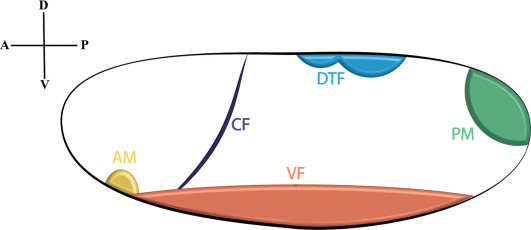
\includegraphics[width = 0.7\linewidth]{chapters/Theory/figures/morphogenic_events.jpg}
    \caption{Summary of the morphogenetic events mapped onto the blastoderm stage embryo. Taken from \cite{gheisari2020gastrulation}. The colored parts are generally seen to be the morphogenetically active during the early part of the embryogenesis}
    \label{fig:enter-label}
\end{figure}

IN OUR SIMULATION: 

The Germ Band is defined as all cells expressing a sufficient YY of the two striped genes \textit{Eve} and \textit{Run} the at the onset of gastrulation. \cite{zallen2004patterned}



\subsection{The Drosophila Gastrulation in detail}
Now, with the details in place, we can get to the main event!
In 1975 Bownes et al. split the development of the fruit fly from fertilised egg to hatched larvae into 17 distinct events.\cite{bownes1975photographic} We will be looking at stages 5 through 7, lasting about 15 minutes. These are characterized by having the first mesoscopic morphogenetic movements and setting the stage for all morphology to come! 

The Drosophila morphogenesis consist of a series of interconnected localized cell movements. We will now present an abridged overview (The "Good Parts" Version), roughly ordered in time:
\newpage

\begin{figure}[H]
    \centering
    \vspace*{-1cm}\makebox[\textwidth]{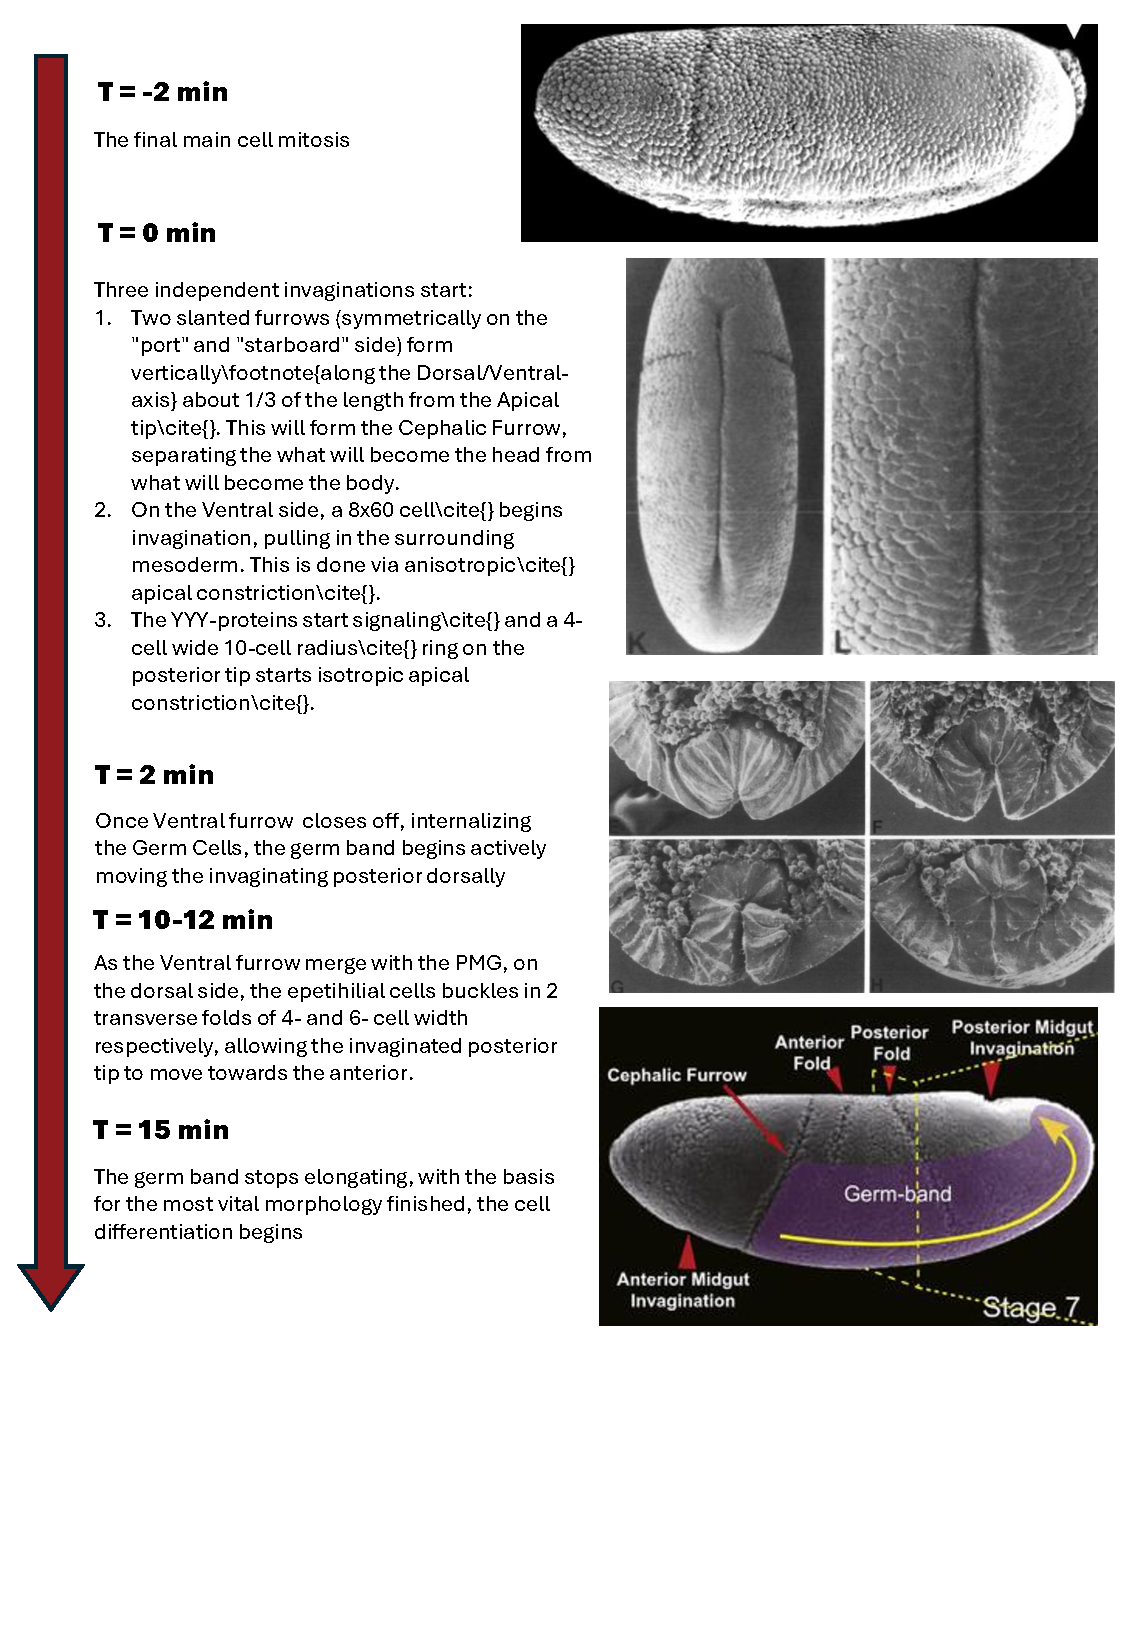
\includegraphics[width=0.8\paperwidth]{chapters/Theory/figures/Timeline.pdf}}
    \caption{Caption}
    \label{fig:big-timeline}
\end{figure}
\newpage
\addtocounter{figure}{-1}
\begin{figure} [t!]
  \caption{(Previous page.) \\ A somewhat comprehensive explanations of the most important past of the initial parts of the gastrulation.
  }
\end{figure}
\vspace*{5cm} 
\textit{This page is intentionally left blank so the previous page can be taken and kept as a cheat-sheet for later referencing. }
\newpage
\section{Previous attempts at simulation?}
While in silico models has provided multiple working examples of all the aforementioned embryogenesis events, their interplay has proven hard to study.

Mainly finite-element simulations have dominated the field when studying the physics of tubologenesis, tissue-folding etc.  

This all leads us to the star of the show:

\section{The Model}
The model is built around simply simulating the movement of the center of mass of the cells along with their individual orientation. 

As described in \cite{} and \cite{}, the model is based on the following intercellular potential:

\begin{equation}
    V_{ij}=e^{-r_{ij}}-A_{ij}e^{-r_{ij}/\beta}
\end{equation}

Where $r_{ij}$ is the distance between two cellsm $A_{ij}$ is a attraction factor what will be explained later, and $\beta$ is a constant (usually 5, which is very constant). 

Where the individual cell wants to minimize the quantity 
\begin{equation}
    U_i = \sum_j V_{ij}
\end{equation}
Here the sum over $j$ is over all Line of sight/Voronoi neighbors, which should remind you of the nearest neighbor protein connections in Figure \ref{fig:mysosinMeshwork}. 


For $A_{ij}=1$ (we will soon expand on this term), the potential simply looks akin to a Yukawa/YYY potential and can be seen in Figure \ref{fig:potential} 
\begin{figure}[H]
    \centering
    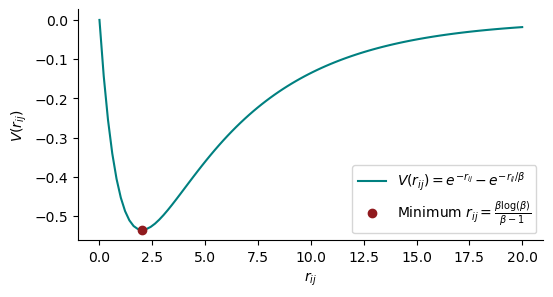
\includegraphics[width=0.8\linewidth]{chapters/Theory/figures/potential.png}
    \caption{The potential well our point particles lie in, with the minimum (i.e. effective cell size) drawn in. Here we also see the role of $\beta$ as responsible for regulating the relaxation-distance}
    \label{fig:potential}
\end{figure}

As we estimate the cells to move slowly and in a friction-filled viscous YYY (the low Reynolds-regime), so each timestep the cells move as subjects to overdamped dynamics:

\begin{equation}
    \frac{d \bar{x}_i}{d t}=-\frac{d V_i}{d \bar{x}_i}+\eta \hspace{1.5cm}|\hspace{1.5cm}  \bar{x} \in \{\bar{r}, \bar{p}, \bar{q}\}
\end{equation}

where $\eta$ is uncorrelated Gaussian noise.
$\cdots$\\
Now, just like nature, we will want to break some symmetries to allow for interesting morphologies to emerge.\\
The principal idea is to elevate the Apical-Basal and Planar-Cell polarities (as described in previous sections) by seeing them as explicitly stated polarization vectors with rules for self- and neighbor interaction (mechanotransduction as described in section \ref{sec:theory-polarity})
Introducing a more complicated $A_{ij}$-parameter we see it as a sum of four terms
\begin{equation}
    A_{ij}=\sum_{n=0}^{3}\lambda_n  S_n
\end{equation}



As previously mentioned the interplay between cell-polarisation and physical orientation goes both ways. This motivates the following four terms which I will quickly explain one by one:
\begin{subequations}
\begin{align}
S_0&=1\label{eq:s0}\\
S_1&=\left(\hat{p}_i \times \hat{r}_{i j}\right) \cdot\left(\hat{p}_j \times \hat{r}_{i j}\right)\label{eq:s1}\\
S_2&=\left(\hat{p}_i \times \hat{q}_{i}\right) \cdot\left(\hat{p}_j \times \hat{q}_{j}\right)\label{eq:s2}\\
S_3&=\left(\hat{q}_i \times \hat{r}_{i j}\right) \cdot\left(\hat{q}_j \times \hat{r}_{i j}\right)\label{eq:s3}
\end{align}
\end{subequations}

As can be seen, the dot-product of cross products are used multiple times. This configuration can be understood for $\left(a \times b\right) \cdot\left(c \times d\right)$ as "keep a and c, and b and d respectively parallel, while keeping a and b, and c and d internally perpendicular".\\


\begin{figure}[H]
    \centering
    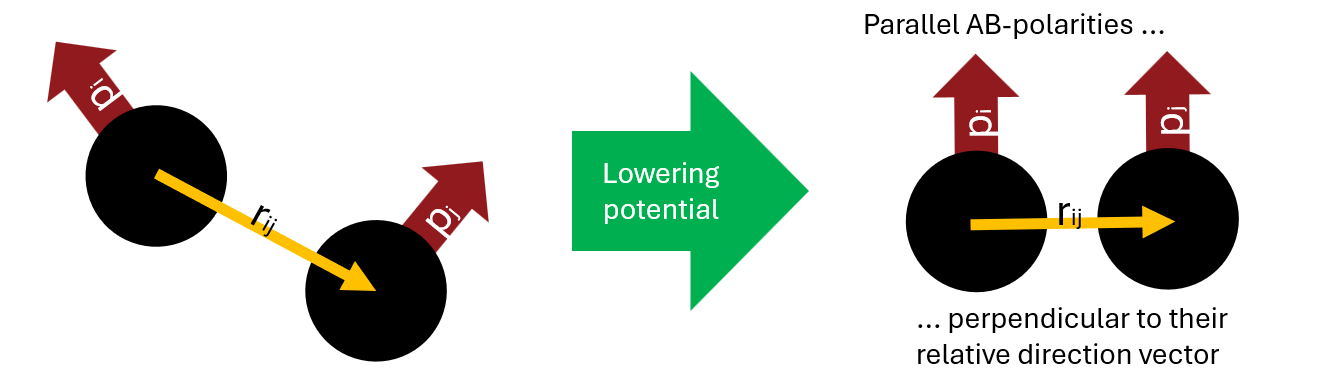
\includegraphics[width=0.3\linewidth]{chapters/Theory/figures/explainS1.png}
    \caption{A visual help for understanding the influence of the $S_1$-term (Equation \ref{eq:s1}). The orange arrow is the AB-polarity and the blue circles representations of the positions of the cells.}
    \label{fig:explain-S1}
\end{figure}

$S_0$ is 1 and is there to allow for constant non-polar attraction.
$S_1$ (Equation \ref{eq:s1}) makes sheets, keeping the Apical and Basal sides of the cells parallel, but also perpendicular to vector between the cell centers. \\
$S_2$ (\ref{eq:s2}) keeps the Apical-Basal and Planar-Cell-polarities perpendicular within each cell, but aligned across cells.\\
$S_3$ (\ref{eq:s3}), finally, is lowest when the Planar-Cell-polarities are aligned but perpendicular. In the realm where this dominates, the cell sheets created by $S_1$ are exchanged for lines of cells perpendicular to their PCP-vectors. $S_3$ is the main driver of in-plane motion through 'convergent extension'-like behaviour  (Section \ref{sec:ConvergentExtension}).\\
If the constraint $\sum_{n=1}^{3}\lambda_n=1$ is not fulfilled, the effective cell size is not constant.\\

\textbf{important} the $\hat{p}_i$'s and $\hat{q}_i$'s are normalized each frame.

$S_3$ allows for convergent extension, Now, we would like to emulate apical constriction (Section \ref{sec:ApicalConstriction}) this is done via \textbf{Wedging}\\

Changing the 

\begin{equation}
    \tilde{{p}}_i = \frac{\hat{p}_i-\alpha \widehat{{r}}_{i j}}{|\hat{p}_i-\alpha \widehat{{r}}_{i j}|} 
\end{equation}
A similar expression can be made for anisotropic wedging, taking  $\hat{q}_i$'s into account.

As is described in the original paper:\\ 
"The final shapes are robust to noise but sensitive to initial and
boundary conditions"\\




Now all cells are defined through a cell type, which simply means they have a $\lambda$-array and a $\alpha$ associated with them.

As we have about 5000 cells, this effectively gives 25000 parameters.

To combat this, we again look to nature and the patterning she has already created for us. In \cite{shinyDVEX} they map out the relative gene expression for the drosophila embryo and YYYY. We can then take YYY and project them onto our embryo. \todo{make sound harder}. Taking these found and cross referencing with 

In appendix \ref{somwehere}\todo{make} the exact choices made and justifications can be seen.

We now set up a pipeline allowing for a simple run to go [something like this]:

\begin{lstlisting}
# Start a new egg from a relaxed base shape
GE = GeneExpression("base_shape.hdf5")

# combine genes through [and, or, not]
twist_and_snail = GE.and_gene(GE.gene("twi"), GE.gene("sna"))

# Make every cell expressing this at least 20% cell type 2 
GE.add_expression(twist_and_snail, 0.2, 2)  # Ventral Furrow

# save and run simulation
GE.save("name_of_expression_profile",)

\end{lstlisting}

Given we choose 4 different cell types and no non-polar interaction, we have cut down to only have 16 parameters. Locking in the $\lambda$'s lowers this even further to about 6 parameters. 

Is it possible to accurate simulate the origin of life using 6 parameters? Read on to find out!

A note for reading on:\\
As the model is purely point-based, whenever we speak of inter-cellular junctions, neighbors, areas or angles, everything is inferred from the modeled point cloud and Voronoi-neighbors.

\section{Implementation}
The gradient is calculated via an automatic differentiation engine (The PyTorch-framework specifically) and the simulation time steps are calculated via Euler integration.

This is not interesting to read about, so extensive notes on the actual implementation along with pseudocode, can be found in Section \ref{App:Code} in the Appendix.

